%Chap 4b pag 5
\definecolor{Purple}{RGB}{153,0,153}
\definecolor{Pink}{RGB}{255,0,131}
\begin{frame}{Ejemplo: n-reinas}
Ponga \textcolor{Purple}{n}\, reinas en un tablero \textcolor{Purple}{n x n} sin poner dos reinas en la misma fila, columna o diagonal.\\
Mueve a una reina para reducir el número de conflictos.\\
\begin{figure}
    \centering
    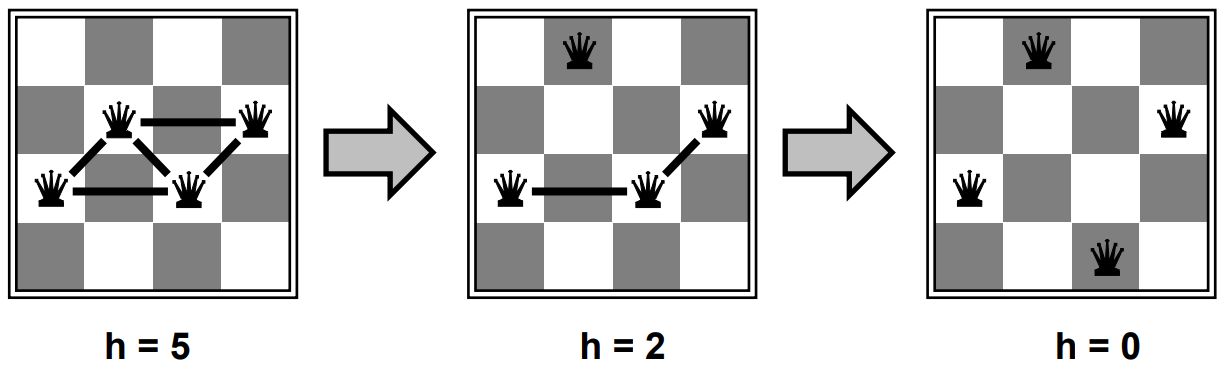
\includegraphics[width = 80mm, scale = 1]{images/4b5_image.PNG}
\end{figure}
Casi siempre resuelve problemas de \textcolor{Purple}{n}-reinas casi instantáneamente para \textcolor{Purple}{n} muy grande, por ejemplo, \textcolor{Purple}{n = 1 millón}
\end{frame}